\documentclass{article}
\usepackage[preprint]{neurips_2023}


\usepackage[utf8]{inputenc} 
\usepackage[T1]{fontenc}    
\usepackage{hyperref}       
\usepackage{url}            
\usepackage{booktabs}       
\usepackage{amsfonts}       
\usepackage{nicefrac}      
\usepackage{microtype}      
\usepackage{xcolor}         
\usepackage{amssymb}
\usepackage{amsmath}

\usepackage{graphicx}
\usepackage[verbose]{placeins} 

\title{Analysis on Reinforcement Learning Methods on Navigation in a Dynamic Environment}


\author{
	Callum Hendry: 100970932\\
	\texttt{callumhendry@cmail.carleton.ca}
	\And
	Jason Dunn: 101140827\\
	\texttt{jason.dunn@carleton.ca}
	\And
	Ujan Sen: 101171605\\
	\texttt{ujansen@cmail.carleton.ca}
	\And
	Uvernes Somarriba: 101146733\\
	\texttt{uvernes.somarribacast@cmail.carleton.ca}
}


\begin{document}
	
	
	\maketitle
	
	\section{Introduction}
	Navigation within a dynamic environment towards objective targets is a complex task requiring both the proper adherence to environment rules, such as following stop light rules within the context of road travel, and path planning capabilities for determining an efficient route across all targets. In this work, we explore various reinforcement learning approaches for the automatic navigation of such dynamic environments. Specifically, we devise RL algorithms to train agents capable of visiting all targets of interest in some arbitrary sparse graph, in both an efficient and well-behaved manner, given a variety of input parameters about the environment network state. This is a simplified simulation that is analogous to simulating dynamic pathing around a road network. The various reinforcement learning methods we devise are evaluated for effectiveness, efficiency, and adaptability.
	\\ \\
	Devising strong solutions towards autonomous navigation has immense value. The most immediate benefit is that this would facilitate the incorporation of self-driving cars within the real-world. It has been observed in several other domains for agents to achieve superhuman performance, and if this were to extend to vehicle navigation, it would yield a reduced number of incidents on the road. This reduction in accidents would lead to fewer car-related deaths and injuries per year, thereby indirectly saving an immeasurable number of lives. In addition, self-driving cars may reduce the waiting times for deliveries, such as for packages or medication. Outside the context of the roads, it may be possible to incorporate autonomous navigation to other tasks such as the robotic navigation of a medical instrument to an anatomy of interest during a medical procedure, to provide aid to practitioners. Thus, there are tremendous benefits to be sowed from work in autonomous navigation. 
	\\ \\
	The paper proceeds with a discussion of pre-existing research in dynamic navigation, an explanation of our specific task environment, our devised RL methods, their resulting performances, and a discussion of these results. We then conclude with some closing remarks.
	
	\section{Related Work}
	
	There has been previous research in autonomous navigation of dynamic environments. 
	
	[-1] introduces Globally Guided Reinforcement Learning (G2RL), a novel approach to robot navigation in a dynamic environment, combining a global guidance approach, using traditional algorithms such as A* search, with localized RL suitable for avoiding dynamic obstacles.
	
	[-2] discusses an RL approach to the traveling salesman problem in a dynamic environment, where stochastic factors are present. Deep RL with an attention model is used, incorporating encoder-decoder architectures, capable of handling changing environment conditions such as traffic. 
	
	[-3] implemented a framework called MCAL (Mobile robot Collision Avoidance Learning) wherein the agent acquires its current state information from a GPS, locating it relative to the target, but they also added a Look Ahead Point (LAP), calculated by its Lidar system, which is a short term goal. If the agent encounters a dynamic obstacle that doesn’t show up on the GPS, it uses a RL system where the further away it moves from the LAP, the higher negative reward it receives, discouraging moving too far off target. However, it receives a much more substantial negative reward if it collides with the obstacle.
	
	[-4] deals with multi-agent path finding, where numerous agents must travel to their own locations in a way such as to not conflict with one another. The developed algorithm PRIMAL combines RL and imitation learning. It is particularly of value in environments where multiple delivery drivers operate simultaneously in the same city.
	\\
	****I think we need 4 more briefly mentioned papers here. I don't think the papers linked in our approaches are the same thing. In specs: \\
	"Provide a brief review of prior work on this problem (at least 5 papers)"
	****
	\section{Environment Setup}
	
	An RL environment is typically modelled as a Markov Decision Process, which is comprised of a state space, action space, its transition probabilities and reward structure.
	
	The environment we modelled for this task simulated a road network environment, and it supported the use of an underlying, arbitrary graph structure $G = (V, E)$, where V is some set of nodes and E is the set of edges between nodes, defining which transitions are possible from a given node. For each $v\in V$, it is either a regular or traffic node, where a traffic node toggles between a green and red light after a certain number of time steps. At the start of an episode, the agent begins at a random node and the environment contains a target at one or more vertices. The episode terminates once the agent has picked up all nodes, if an action leads to a crash outcome or a cutoff max number of episodes have passed.
	
	The specific road network used in training and evaluation was a 5x5 grid world, where each node had a 0.10 probability of containing a target, represented as yellow. Non-target nodes had a 0.6 probability of being traffic lights, represented as toggling red and outer circles. The agent, placed randomly at a non-target node, was represented in blue. See Figure 1 below for a random instance of the grid world.
	
	\begin{figure}[hbt!]
		\centering
		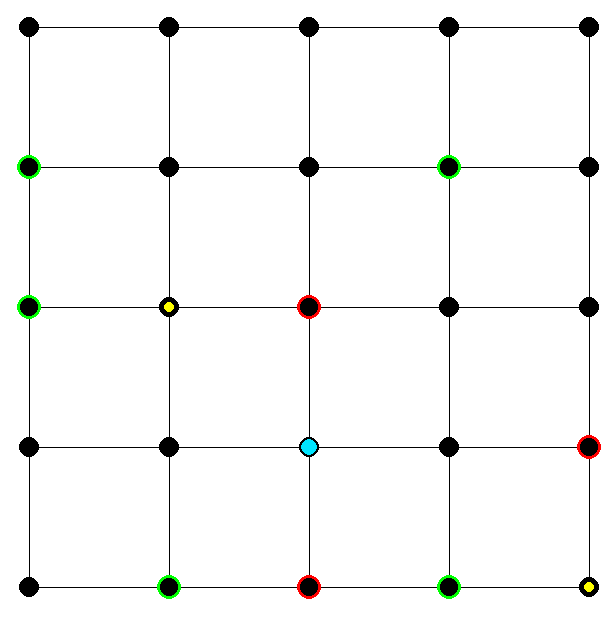
\includegraphics[scale=0.5]{grid-world.png}
		\caption{caption here}
		\label{fig:grid-world.png}
	\end{figure}
	\FloatBarrier 
	
	The original state space was a 4-tuple of the form: (A,A',Targets,Traffic). A and A' are integers representing the current and previous index of the node the agent was at. Targets is a |V|=25 Boolean vector with $V_{i}=1$ if $V_i$ contains a target and zero otherwise. Traffic is a Boolean value which is 1 if and only if the current node is a traffic node and it is a red light.
	
	The agent's action space was discrete and consisted of 5 possible actions: move left, right, up, or down, or stay at current node. The edges corresponding to out of bound actions pointed back to the same node.
	
	The original reward structure, which was slightly modified in certain implementations, involved both deterministic and stochastic components. If the agent picked up a target, the target disappeared from the environment and the agent received a reward of +1. If the agent took an action going out of bounds, the reward was -2.0 and the episode terminated. If the agent performed a U-turn at a non-red light, where a U-turn action was detected by considering the angle between the previous and next node, there was a 0.8 probability the agent received -2.0 reward and the episode terminated. Furthermore, if at a red stop light and the agent turned right, left, straight, or back, with probabilities 0.4, 0.8, 0.9, and 0.95, respectively, a reward of -5.0 was given along with episode termination. In all other cases, such as legal movement to a non-target node, a reward of 0 was given.
	
	\section{Methods}
	\subsection{Proximal Policy Optimization (PPO)}
	\label{ppo}
	
	Proximal Policy Optimization (PPO) was introduced in 2017 [1] and has achieved widespread success in the realm of reinforcement learning. It was a successor to Trust Region Policy Optimization (TRPO) introduced in 2015 [2] which used stochastic gradient ascent by using a trust region constraint to regulate between the old policy and the new updated policy. PPO is considered state-of-the-art and is the default reinforcement learning algorithm used at OpenAI because of its ease of use and significantly better and faster performance than its counterparts. 
	
	The biggest difference between PPO and TRPO is that PPO uses a clipping function which effectively ensures that the new learned policy does not deviate more than a certain amount from the old policy. This is done by first calculating two different sets of surrogates for the policy network. The objective for PPO is calculated as follows [1]:
	
	\begin{center}
		$L_{\theta} = \mathbb{E}_{t}[min(r_{t}({\theta})A_{t}, CLIP(r_{t}({\theta}), 1-\epsilon, 1+\epsilon)A_{t})]$
	\end{center}
	
	For the surrogates, the ratios are first calculated between the predicted actions at the current state given the old policy and the new predicted actions. The first surrogate is calculated by weighting the ratios by the calculated advantages. The second surrogate is calculated in a similar way except the ratios are first clipped between 1 - $\epsilon$, and 1 + $\epsilon$ where epsilon is defined as the clip ratio, and then weighted with the advantages. The loss is then defined to be the minimum of these surrogates.
	
	Advantages are calculated using Generalized Advantage Estimation (GAE) introduced in 2015 [3]. GAE is an improvement upon traditional advantage estimation methods because of the introduction of the $\lambda$ term which allows a trade-off between bias and variance. A $\lambda$ of 0 reduces GAE to a one-step estimation which is just standard advantage estimation whereas a $\lambda$ of 1 considers rewards infinitely into the future. It takes into consideration the temporal difference of not only the immediate rewards but also the expected future rewards. The formula for GAE calculation is as follows [3]:
	
	\begin{center}
		$\hat{A}^{GAE}_{t} = \sum_{k=0}^{\infty}(\gamma.\lambda^{k}).\delta_{t+k}$
	\end{center}
	\begin{itemize}
		\item $\hat{A}^{GAE}_{t}$ is the GAE at time step $t$
		\item $\gamma$ is the discount factor
		\item $\lambda$ is the GAE parameter, the tradeoff between bias and variance
		\item $k$ is the time step offset
		\item $\delta_{t+k}$ is the advantage at time step $t+k$ calculated using the one step standard advantage calculation
	\end{itemize}
	
	The intuition behind choosing PPO is the same as TRPO: "being safe". Since the loss function is defined as the minimum of the two surrogates, the objective becomes a lower bound of what the agent knows is possible. It approaches the task being a pessimist, which has often times proved to be more beneficial than being optimistic with little chances of recovery. TRPO's objective function achieves a similar thing but is quite different in computation [2].
	
	\begin{center}
		$L_{\theta} = \mathbb{E}_{t}[D_{KL}(\pi_{\theta_{old}}(.|s_{t}) || \pi_{\theta}(.|s_{t}))] \leq \delta$
	\end{center}
	
	The benefit PPO gives over TRPO is the usage of clipped ratios and the surrogates. TRPO enforces a strict trust region constraint where the KL-divergence between old policies and new policies is small enough, within a parameter $\delta$ leading to a second-order optimization problem [2][4]. PPO effectively does the same thing using the clipped ratio and taking the minimum of the surrogate losses resulting in a first-order optimization problem. This leads to PPO utilizing fewer computation resources while providing better results.
	
	The PPO implementation was performed using the library stable\textunderscore baselines3 available  \href{https://stable-baselines3.readthedocs.io/en/master/}{here}. It ran with default arguments as described in the documentation.
	
	\subsubsection{Environmental Considerations}
	\label{considerations}
	The environment was modified and the results for each modification of the environment is mentioned in the Results section.
	\begin{itemize}
		\item The targets were reduced from multiple to single. 
		\begin{itemize}
			\item Relative directionality from agent to target introduced using a 4-element 1D array
		\end{itemize}
		\item Running traffic lights, making u-turns, and going out of bounds were always penalized instead of it being probabilistic
		\item All penalized actions penalized to the same amount
	\end{itemize}
	
	\subsection{Advantage Actor Critic (A2C)}
	\label{a2c}
	A2C is an actor critic algorithm which was created by the need to address the limitations of its predecessor, the Asynchronous Advantage Actor-Critic (A3C) algorithm, particularly regarding the asynchronous nature of A3C which could lead to non-optimal convergence due to delayed updates from its multiple worker agents.[5] The A2C algorithm modifies this approach by implementing synchronous updates, which means it waits for each of its multiple agents to finish their experience trajectories before it updates the model. This change leads to more stable and consistent learning, as all updates are based on the most current data.
	
	A pivotal element in A2C is the advantage function, denoted as \( A(s, a) \). This function is defined as the difference between the action-value function and the state-value function: 
	
	\begin{center}
		$A(s, a) = Q(s, a) - V(s)$
	\end{center}
	
	The advantage function quantifies the relative benefit of an action \( a \) in a state \( s \) compared to the average action at that state. By focusing on the advantage function, A2C targets learning on actions that are more beneficial than average, thereby enhancing the efficiency of the learning process. The policy, guided by the Actor, is updated using a gradient ascent approach on the expected return. The formula is expressed as: 
	\begin{center}
		$\theta \leftarrow \theta + \alpha \nabla_{\theta} \log \pi(a | s, \theta) A(s, a)$
	\end{center}
	
	Simultaneously, the Critic is updated to improve its estimates of the state-value function. This usually involves minimizing the difference between the estimated values and the actual returns, enhancing the accuracy of the Critic's evaluations.
	
	Some reasons for using A2C with our particular problem is that it works well with discrete environments, and the advantage function reduces the negative impact of high variability between individual episodes, which was very likely in our environment due to the random placement of targets, and traffic lights. It has also been used in other traffic problems.
	
	
	\subsection{Double Deep Q-Learning}
	
	An alternate function approximation approach to PPO was explored via the use of a Double Deep Q-Learning Architecture, introduced in [X].
	
	In tabular Q-learning, estimates of the optimal action-values are updated based on Bellman's optimality equation [Y]:
	\\
	\begin{center}
		$Q(S_{t}, A_{t}) \leftarrow Q(S_{t}, A_{t}) + \alpha\cdot\delta_{t}$
	\end{center}
	
	Where $d_{t}$ is given by [Y]:
	
	\begin{center}
		$d_{t} = R_{t+1} + \gamma\max_{a'}Q(S_{t+1}, a') - Q(S_{t}, A_{t})$
	\end{center}
	
	However, this requires storage of the estimates for each state individually and good estimates can only be acquired for a state if it is visited sufficiently many times. Acquiring adequate estimates in this manner is infeasible for large state spaces, including for the task examined in this paper, so a function approximation approach must be taken.
	
	Q-learning via function approximation requires the learning of a function able to map the feature representation of states to their associated action-values under an optimal policy. In deep Q learning [X], the learned function is a deep neural network, and its performance at estimating values, measured by some loss function, is improved via some propagation algorithm.
	
	In our implementation, the cost function calculates the error between samples by mapping $d_{t}$ using the Huber Loss function [Z]:
	
	\begin{equation}
		L(\delta)=
		\begin{cases}
			\frac{1}{2}\delta^{2} & \text{if  } |\delta| \leq 1\\
			|\delta| - \frac{1}{2} & \text{otherwise} 
		\end{cases}
	\end{equation}
	
	The specific architecture consisted of a fully connected, 3-layer network using the reLU activation function to introduce non-linearity.
	
	The portion resulting in the name of a 'Double' DQN is that there were two networks utilized [X]. The primary network was the policy network and it was responsible for the prediction of the action-values from the current state. The secondary network was called the target network and it was utilized in computing the action-values of the subsequent state, which is a necessary calculation in computing the target and thereby finding the loss when updating. The weights of this network were made to slowly update to the weights of the policy network, where the policy network weights may change in a different direction. This stabilizing of target values has shown to lead to better model performance [X]. Another trick utilized for the improvement of agent results was the use of replay memory, in which the implementation stored the last ten thousand transitions and sampled from this storage during training.
	
	The training portion of the implementation was done twice, once for the agent in the original environment with multiple targets, and once for the agent in the same environment but with the simplification of only a single target being present.
	
	The reasoning behind using a DQN-approach was that such algorithms are well-suited to discrete environments, and a comparison of performance could then be done with actor-critic methods PPO and A2C.
	
	The Double DQN implementation was conducted by following the PyTorch tutorial for Deep Q-learning (available \href{https://pytorch.org/tutorials/intermediate/reinforcement_q_learning.html}{here}), and all hyperparameters were kept the same.
	
	
	\subsection{Planning Meta-Agent}
	\label{planning}
	In this design architecture, an agent consists of two parts. First, it has an agent trained for navigating from a given state to another given state with the maximum reward. However, this agent alone has limited usefulness as it does not have any reasonable way to handle longer runs with multiple targets. To solve this problem another component is added to the agent which is specialized in forming long term plans. Essentially, these components treat the environment as a fully connected graph, and it is able to go from any node to any other node with a single action. It is able to do this as the designer knows that the navigation agent is able to move from any node to any other node in some number of actions.
	
	Several different methods were experimented with to try to create a pathing component. It should be noted that these are not restricted to reinforcement learning, as it is worth considering what other options may offer better performance, as reinforcement learning is not suited to all tasks.
	
	\subsubsection{Q-Learning}
	In this approach standard Q-Learning is used based on a complete graph, with the reward going from any node to any other node being equal to the reward obtained by the navigation agent going between those two nodes. For efficiency two abstractions are made: first, this algorithm only tries to solve the travelling salesman problem for the target nodes, as it is not relevant to plan to visit the others, and second it creates a single reward matrix by running the navigation agent several times, then it simply re-uses those rewards. Given a more restricted environment, it may be viable to plan a path since the action space is more limited [Nova 5]
	
	Unfortunately, using the maximum at each step may not end up creating a complete cycle. Thus, the designer must choose some way to select which actions are taken based on the Q-values. Obtaining the true optimal choices from the Q-Values would involve solving the travelling salesman problem on the values themselves, which effectively defeats the purpose of using this method.
	
	\subsubsection{Gradient Descent Neural Network}
	The main difficulty that this method faces is the lack of a clear differentiable loss function, unless one has access to the true outputs they are aiming for. Thus, in order to use this approach one would have to implement a different method first, which defeats the purpose of using this algorithm. The only practical use of this could be to reduce computation time by training it to mimic a good heuristic algorithm.
	
	\subsubsection{Step-Wise Neural Network}
	This approach uses a neural network that takes in the current state, and outputs a softmax probability output of which node the navigation agent should target next. It is possible that this may give good performance eventually, however due to the lack of a meaningful gradient, the only feasible way to train this is to use evolutionary methods.
	
	\subsubsection{Budinich Neural Network}
	This method was an early attempts at using the self-organizing properties of neural networks to produce a single cycle path on some number of points on a 2D plane [Nova 1]. It theoretically achieves this by mapping each input to a point on a ring of output neurons. In order to create a full path it takes in the euclidean position of each node one at a time and then maps it somewhere on the real number line. This method produces better than random results, however the performance is not as good as other methods. In addition, it is unclear how one would generalize this method to non-euclidean spaces.
	
	\subsubsection{Evolutionary Mapping Neural Network}
	\label{evol_nn}
	In this approach a neural network is trained to give each node a point on the one-dimensional number line, where it is trivial to solve the travelling salesman problem. In order to do this, it takes in the entire observation given by the environment, and outputs one decimal number per node. These are then sorted and used as the path. This method would eventually give extremely good results as it can converge to a global minima given enough time. However, the main drawbacks of this method are related to its time performance. Evolutionary methods are extremely slow to converge, and it would need to be retrained whenever any aspect of the environment is changed, such as adding or removing a node.
	
	\subsubsection{Christofides-Serdyukov Algorithm}
	Although this algorithm is typically very effective, it is not well suited to this particular problem as the environment does not meet the requirements to be considered a metric space [Nova 2]. Namely it violates the following conditions: First, the distance from any node to itself is not zero, as there is a penalty for idling. Next, there is no assumption of symmetry. Finally, there is no guarantee that the triangle inequality will hold depending on the quality of the underlying navigation agent. Thus, the usage of this algorithm would be restricted to the Euclidean distances, which misses significant amounts of nuance in the environment.
	
	\subsubsection{Nearest Neighbour}
	\label{nearest_neighbour}
	This is essentially the simplest method one could use to obtain a reasonable path. It works by starting with a random node and constructing a complete path by iteratively selecting the nearest node that has never been visited as the next node in the path. It has no performance guarantees, however it should perform reasonably well on most inputs. [Nova 4] This method is simple to adapt for our meta agent, as we can construct a distance matrix between every pair of nodes.
	
	\subsubsection{Ant Colony Optimization (ACO)}
	\label{aco}
	This method uses a large population of simple agents. For each agent, they start at a random node, and need to complete one full cycle. Then they apply a value of $\frac{1}{cycle length}$ to the action it took along each step of its path. Then, future agents are able to use this pheromone trail to probabilistically select the next node they go to. Since lower cycle lengths give a higher value, the ants will eventually produce a good quality approximation of the shortest path using a time proportional to the number of agent iterations. This produces very good results, and works well in the non-euclidean space as it solely relies on cycle lengths, and not any other property of the environment. [Nova 3]
	
	Overall, although it may be possible to train a planning agent using reinforcement learning, in practice hand crafted algorithms are still able to achieve superior results.
	
	\section{Results}
	\label{results}
	In this section we will discuss the results for the various implemented algorithms:
	
	\begin{table*}[h]
		\centering
		\caption[]{Results for PPO}\label{Results for PPO}%
		\begin{tabular}{cccccc}
			\toprule
			Target & Reward Type & Reward Scaling\footnotemark[1] & Agent Score\footnotemark[2] & Random Score\footnotemark[2] & Train Time\footnotemark[3]\\
			\midrule
			Single &  Deterministic & Same & 875 & -396 & 15\\
			Single & Deterministic & Different\footnotemark[4] & 935 & -369 & 15\\
			Single & Probabilistic & Different & 890 & -334 & 20\\
			\midrule
			Multiple & Deterministic & Same & 205 & -405 & 20\\
			Multiple & Deterministic & Different & 379 & -390 & 20\\
			Multiple & Probabilistic & Different & 255 & -410 & 30\\
			\bottomrule
		\end{tabular}
		\label{tab: PPO_Table}
	\end{table*}
	\footnotetext[1]{Only negative rewards are altered, positive rewards remain the same}
	\footnotetext[2]{Scores are approximately out of 1000 for single target - Approximate because there is additional positive reward for stopping at traffic light}
	\footnotetext[3]{In minutes}
	\footnotetext[4]{Stop at green: -2; Stop at node that is not traffic light: -2; Everything else: -5}
	
	\begin{table*}[h]
		\centering
		\caption[]{Results for A2C}\label{Results for A2C}%
		\begin{tabular}{cccccc}
			\toprule
			Target & Reward Type & Reward Scaling\footnotemark & Agent Score\footnotemark & Random Score\footnotemark & Train Timesteps\footnotemark\\
			\midrule
			Single &  Deterministic & Same & 865 & -417 & 10,000\\
			Single & Deterministic & Different\footnotemark & 899 & -301 & 10,000\\
			Single & Probabilistic & Different & 921 & -407 & 10,000\\
			\midrule
			Multiple & Deterministic & Same & 220 & -366 & 20\\
			Multiple & Deterministic & Different & 262 & -233 & 10,000\\
			Multiple & Probabilistic & Different & 73 & -257 & 10,000\\
			\bottomrule
		\end{tabular}
		\label{tab: A2C_Table}
	\end{table*}
	
	`   \begin{table*}[h]
		\centering
		\caption[]{Results for Double DQN}\label{Results for PPO}%
		\begin{tabular}{cccc}
			\toprule
			Target & Agent Return & Random Return & Training Episodes \\
			\midrule
			Single & 326 & -301 & 1000 \\
			Multiple & 23 & -305 & 10000 \\
			\bottomrule
		\end{tabular}
		\label{tab: PPO_Table}
	\end{table*}
	
	\section{Discussion}
	\label{discussion}
	From the results, it is clear that for PPO, the more complex the environment becomes, the worse the agent performs. This is expected as it is quite difficult to find an optimal solution to our problem considering how the environment behaves. When there is a single target, there does not seem to be large difference in performance. The higher score for different reward scaling compared to same can be attributed to the fact that when it makes mistakes, the penalty is lower in the different reward scaling scenario, which is coincidentally also the case for the multiple targets scenario. It is worth noting that the total score for multiple targets is difficult to say since the number of targets is not fixed but it is more than 1000 since there is always at least one target.
	
	Table 2 illustrates the results for the actor-critic implementation. This A2C implementation was using the stable\_baseline3 package. It ended up yielding far better results than those shown during the demo which was a different implementation of A2C.
	
	Table 3 showcases the performance of the DQN implementation in the context of the original environment, where reward structures are kept stochastic and scaled, but two separate agents were trained. One agent was trained for multi-target environments and the other for single targets. As in all other implementations, performance worsened when the environment was unrestricted to multiple targets. Upon further investigation for the DQN implementation specifically, it appeared the optimal policy learned by the agent was to remain stationary, so this implies the method was prone to poor finding poor local minima. In addition, DQN performed worse than A2C and PPO. In particular, it showed far slower convergence time towards optimal behaviour. It is suspected this gap may be reduced if a search is done for better hyperparameters.
	
	An interesting idea would be to fix the traffic lights instead of randomly initializing them. This seems quite intuitive and in fact, could even be considered closer to reality since if the environment is a representation of an urban city setting and we consider that it is the same city, traffic lights and their locations will not suddenly change. And even if they do change, they should remain consistent for a significant time once they do. Perhaps this is an avenue worth exploring where traffic lights are initially fixed but can randomly change after a certain amount of time steps. 
	
	In both the single target and the multiple target scenario, the agent performs worse than the best agent when penalties are probabilistic which makes sense since this is a difficult environment dynamic to learn. Whenever probabilistic elements are introduced into the environment dynamics, it makes training significantly tougher since even though it might revisit a state and take the same action as it did last time, it might receive a different reward.
	
	Furthermore, it is worth noting that multiple targets yield worse results than singular targets. This is expected because of the fact that when there are multiple targets, there is no way to encode direction, which was something we were able to do when there was a single target. For example, if there was a single target, we had relative directionality indicating where the target was. But when there are multiple scattered targets, this sort of information is difficult to encode. 
	
	Given more time and resources, we would like to implement the planning agent that works in tandem with our navigation agent. This could be achieved via the various methods outlined under \ref{planning} with the most promising ones being Nearest Neighbour \ref{nearest_neighbour} and ACO \ref{aco}. One could argue that an evolutionary mapping neural network \ref{evol_nn} would also be effective to use on top of our navigation agent because of its eventual convergence to a global minima, but training it is non-trivial.
	
	Thus, the optimal way to solve our environment would be using a good planning agent that picks the next target for our navigating agent that has been trained using PPO, effectively reducing the state space from having multiple targets to a single target once again, allowing us to encode direction again. We can say with confidence that this would be optimal since this is pretty close to how humans would operate with this environment and furthermore, seeing how well PPO performs on the single target scenario, we can say with high certainty that this will indeed provide optimal results.
	
	Given more time and resources, we would also like to test out more scenarios including various combinations of the scenarios mentioned in \ref{considerations} along with \ref{planning}. We would also like to test various reinforcement learning algorithms and their performance if the targets had priorities assigned to them. We would also like to add pedestrians and random events in the environment and evaluate performance.
	
	\section*{References}
	
	
	[1] Schulman, J., Wolski, F., Dhariwal, P., Radford, A., \& Klimov, O. (2017). Proximal Policy Optimization Algorithms. arXiv preprint \href{https://arxiv.org/abs/1707.06347}{arXiv:1707.06347}.
	
	[2] Schulman, J., Levine, S., Moritz, P., Jordan, M. I., \& Abbeel, P. (2017). Trust Region Policy Optimization. arXiv preprint \href{https://arxiv.org/abs/1502.05477}{arXiv:1502.05477}.
	
	[3] Schulman, J., Moritz, P., Levine, S., Jordan, M., \& Abbeel, P. (2018). High-Dimensional Continuous Control Using Generalized Advantage Estimation. arXiv preprint \href{https://arxiv.org/abs/1506.02438}{arXiv:1506.02438}
	
	[4] Wang, Y., He, H., Wen, C., \& Tan, X. (2020). Truly Proximal Policy Optimization. arXiv preprint \href{https://arxiv.org/abs/1903.07940}{arXiv:1903.07940}.
	
	[5] Mnih, V., Badia, A. P., Mirza, M., Graves, A., Lillicrap, T., Harley, T., Silver, D., \& Kavukcuoglu, K. (2016). Asynchronous Methods for Deep Reinforcement Learning. arVix preprint \href{https://arxiv.org/abs/1602.01783}{arXiv:1602.01783}.
	
	[X] van Hasselt, H., Guez, A., \& Silver, D. (2016). Deep Reinforcement Learning with Double Q-Learning. Proceedings of the AAAI Conference on Artificial Intelligence, 30(1). https://doi.org/10.1609/aaai.v30i1.10295
	
	[Y] RL textbook
	
	[Z] Huber Loss. https://arxiv.org/pdf/2108.12627.pdf 
	
	[Nova 1]
	M. Budinich, ‘A self-organizing neural network for the traveling salesman problem that is competitive with simulated annealing’, Neural Comput, vol. 8, no. 2, pp. 416–424, Feb. 1996.
	
	[Nova 2] N. Christofides, “Worst-case analysis of a new heuristic for the travelling salesman problem,” Graduate School of Industrial Administration, 1976. Accessed: Dec. 08, 2023. [Online]. Available: https://apps.dtic.mil/dtic/tr/fulltext/u2/a025602.pdf
	
	[Nova 3] R. BV, “Solving Traveling Salesmen Problem using Ant Colony Optimization Algorithm,” Journal of Applied \&; Computational Mathematics, vol. 04, no. 06. OMICS Publishing Group, 2015. doi: 10.4172/2168-9679.1000260.
	
	[Nova 4] [1]
	D. Rosenkrantz, R. Stearns, and P. Ii, ‘An Analysis of Several Heuristics for the Traveling Salesman Problem’, SIAM J. Comput., vol. 6, pp. 563–581, 09 1977.
	
	[Nova 5]
	Q. Jiang, ‘Path Planning Method of Mobile Robot Based on Q-learning’, Journal of Physics: Conference Series, vol. 2181, no. 1, p. 012030, Jan. 2022.
	
	
\end{document}

